\documentclass{article}
\usepackage[T1]{fontenc} % add special characters (e.g., umlaute)
\usepackage[utf8]{inputenc} % set utf-8 as default input encoding
\usepackage{ismir,amsmath,cite,url}
\usepackage{graphicx}
\usepackage{color}

% UNCOMMENT THE TWO LINES BELOW TO SEE LINE NUMBERS. I think it is better without the line numbers.
% \usepackage{lineno}
% \linenumbers

\title{Chiptune Extension and Generation using Markov chains}

% Three addresses
% --------------
\threeauthors
  {Oscar Sandford} {University of Victoria \\ {\tt oscarsandford@uvic.ca}}
  {Colson Demedeiros} {University of Victoria \\ {\tt cdemedeiros@uvic.ca}}
  {Jae Park} {University of Victoria \\ {\tt jaehyunpark@uvic.ca}}

\sloppy
\begin{document}
\maketitle

\begin{abstract}
Music generation is a well-studied field. Previous attempts at music generation have succeeded in replicating training tracks using various methods involving complex 
time inference models. In this paper we show that simple, but appropriately designed, first and $k$-order Markov models are a sufficient enough machinery to both 
replicate and generate classic 8-bit video game music. 
\footnote{This abstract will be expounded in time, pending study completion and results organized.}
\end{abstract}

\section{Introduction}
Music is typically constructed by humans, for humans. However, machines are becoming more adept at revealing patterns in the way musicians craft their chords. 
This enables humans to create their own music, and then let the machine take over the task of composer. Our project implements models for simple 8-bit music 
generation using temporal inference techniques. In the following section, we explore previous implementations and existing literature regarding music generation. 
Later, we will present techniques for designing generative Markov models to extend music as well as create derivative musical works.

Markov chains model a \emph{sequence of states}. Changes from one state to another are called \emph{transitions} \cite{markov_survey}. Any given previous state can 
have an arbitrary number of possible next states, each assigned its own transition probability. The sum of these transition probabilities for each option must sum 
to 1 \cite{markov_construct}. Markov chains are generative models, consisting of a set of states of size $N$, and a transition matrix of size $N\times N$ to store 
transition probabilities. 

% TODO: add: what are Markov chains? Explain the details as if the reader is the class.

\section{Related Work}
\subsection{Markov Models}
Yanchenko and Mukherjee explored the use of Hidden Markov Models (HMMs) to compose classical music, finding proficiency in generating consonant harmonies, but 
lacking melodic progression \cite{yanchenko_2017}. Indeed, the models were found to learn the harmonic hidden states quite well, in some cases leading to overfitting. 
HMMs have also found use in chorale harmonization, where a given observable melody uses inference to derive hidden harmonies to complement it \cite{allan_2005}. 

Walter and Van Der Merwe's methods involve representing the chord duration, chord progression, and rhythm progression with first or higher-order Markov chains, whereas 
the overlaying melodic arc is represented by a HMM \cite{walter_2011}. This separation works well to reduce the processing power needed for music generation, but the 
independent learning of each component leads to less cohesive compositions. Generating music is generally done by sampling a statistical model \cite{conklin_2003}.
However, we want to create music that does not only simply replicate the training data, but also creates cohesive pieces in a more natural way. 

Shapiro and Huber's approach to music generation simply uses Markov chains, no hidden states \cite{shapiro_huber_2021}. In their work, the states represent sound 
objects with attributes such as pitch, octave, and duration. Their results show that human-composed pieces can be closely replicated using the simpler Markov chains. 
Further, they have attached their implementation in their paper. We will consider this work when constructing our own implementation.

Corrêa and Jungling suggest using Markov chains of different orders to predict classical music. By using stochastic models to analyze different classcal songs and styles,
the computer can even capture subtle and intuitive features such as style of the composer. Although this paper focuses on classcial music and its prediction, the authors 
stress that its application to other music genres should be straightforward \cite{correa_jungling_small_2020}.
The only requirement is a MIDI file with a good quality, as it should be used for Markov chains that can properly estimate the music's pattern.

\subsection{Data Format}
The papers previously mentioned use the MIDI file format to write digital music. This format appears to be the standard for digital music creation \cite{midi_format}. 
One of MIDI's drawbacks is that it cannot store vocals \cite{cataltepe_2007}. This is of no concern to us, as we will only be attempting to generate instrumental 
compositions. Additionally, successful approaches to melody extraction from MIDI files \cite{ozcan_2005} make assurances that this will be an adequate medium for the 
music our models will generate. MusicXML is a standard file format for storing sheet music, just as MP3 is for recordings \cite{musicxml_2022}. As both are commonly used 
standards, we plan to use MusicXML for input data and write our output to MIDI files.

\section{Approach}
After considering the differences between HMMs and simpler Markov models, we have decided to design our generator as a $k$-order Markov process without hidden states, 
since these methods have seen success in recent works \cite{shapiro_huber_2021,correa_jungling_small_2020}. As of now, we have two designs in mind. The first approach 
involves representing a song with a single chain of sound object states, including pitch, octave, duration, and other attributes. An alternative is using $m$ separate 
$k$-order Markov processes, one for each key on a piano used in the song. It will be prudent to consider extending the order of the processes in this case, in order to 
capture the musical patterns more clearly. Otherwise, first-order probabilistic transitions will inevitably make the generated notes very random. Extending the process 
order also hopes to alleviate the generative faults coming from independently trained Markov chains.

\subsection{Timeline}
We expect to have 3 milestones for this project:
\begin{enumerate}
  \item \textbf{Milestone 1} (February 18th): Convert music to MusicXML files using AnthemScore. Devise sound object structure for Markov states or other architecture. 
  Write a parser to transform the MusicXML data to sound objects. 
  \item \textbf{Milestone 2} (March 21st): Apply Markov chain algorithm to the music samples in order to train the model. We plan to refer to various works that we found.
  By this point, our models should be able to replicate the music tracks given as input. By this point our program will be able to extend music.
  \item \textbf{Milestone 3} (April 7th): Tweak the models to generate more original variations. Enhance the quality of the music. Possibly a GUI for aesthetics as well, 
  if time permits.
\end{enumerate}

\subsection{Task Delegation}
In order to figure out the best approach and gather a plethora of sources, we are each looking at various sources related to music data parsing and music generation, 
from theoretical papers to Python libraries. Colson and Jae are finding classic 8-bit tracks that we will use to train our models on. Oscar has set up a GitHub repository 
to include written work as well as source code, and made outlines for the final report. Moving forward, Colson will be responsible for finding and converting music to 
MusicXML format, and designing a parser to turn notes into data. Jae and Oscar will work on designing the sound object states and programming the generative Markov models. 

\subsection{Resources}
\subsubsection{Tools}
Stacher\footnote{https://stacher.io} is a frontend GUI for YT-DLP, which is a command line downloader that can be installed for converting Youtube videos to MP3 files.
While YT-DLP works just fine, Stacher makes it very easy to convert YouTube links to various file formats (MP3, WAV, AAC, etc.) and save them on your current device. This 
is the software we will use to get the songs as MP3 files saved and put into AnthemScore to be converted into XML files.

AnthemScore\footnote{https://www.lunaverus.com/} is a music transcription software that converts WAV, MP3, and other audio formats into sheet music using an advanced 
neural network. The sheet music can then be exported to various other formats such as PDF, MIDI, or XML. The main use of this software is to easily obtain XML files that 
we will use for data in the Markov chains. While AnthemScore is a great tool to aquire relatively true XML files of songs, the artificial intelligence that powers it does 
occasionally miss notes. What this means for us is that without changing the notes that are detected and placed by the AnthemScore software, it may miss notes or sounds 
that exist within the original song. Despite this, as long as it is mostly accurate and the majority of notes are in place, it shouldn't affect the overall process of the 
project. We will avoid songs that don't transform accurately into MusicXML. Preliminary coding will be done in Jupyter Notebooks using Python. 

\subsubsection{Data Sets}
We are planning to use mostly music from various classic video games, including Super Mario Brothers \cite{kondo_2009},
Undertale \cite{fox_2017} and Legend of Zelda \cite{nakatsuka_2009}.

\section{Documentation}
\subsection{Initial Steps}
The first step we took was the decision to move away from the MusicXML format we started with, for a couple of reasons. For one, it required a software called AnthemScore, 
which is a paid service that works by converting MP3 files to MusicXML format. We had originally downloaded it with a one month free trial, and had intended to find a 
selection of songs in that time, and convert them to MusicXML immediately. We decided that this approach was not extensible, as any future progress using this method would 
require the software again to access new data. From here, we landed on MIDI files to use as data instead, as the existing Mido Python library makes accessing the files and 
data easy. This also removed Stacher, the software we had used to turn YouTube links into MP3, as a requirement.

Another thing we had to consider was the complexity of the MIDI files we used as data. For the most part, the code we wrote to interpret the MIDI file data is quite simple, 
capturing things like the time signature, key signature, tempo, as well as the tracks turned into a list of notes. MIDI files can be quite complex, using things like 
system exclusive messages, control change messages, and more. The second issue was related to the creators of the MIDI tracks, and how they decided to implement simultaneous 
notes. Due to the nature of the RTTTL format, notes and rests play in sequence, from start to finish. This means we intended to have each MIDI track be a different part of 
the song, which would then each have its own RTTTL track that would be analyzed. Unfortunately, track creators can also have notes play simultaneously in one track by having 
a new note on message at $time = 0$ following another note on message of a different note. For these kinds of tracks, we simply have to drop one of the notes that is played, 
since we cannot easily separate them, and we cannot have them play simultaneously in RTTTL format. This, along with the more unique MIDI messages present in some songs, are 
the two main restrictions to our implementation and the tracks we have used as data. \\

\frame{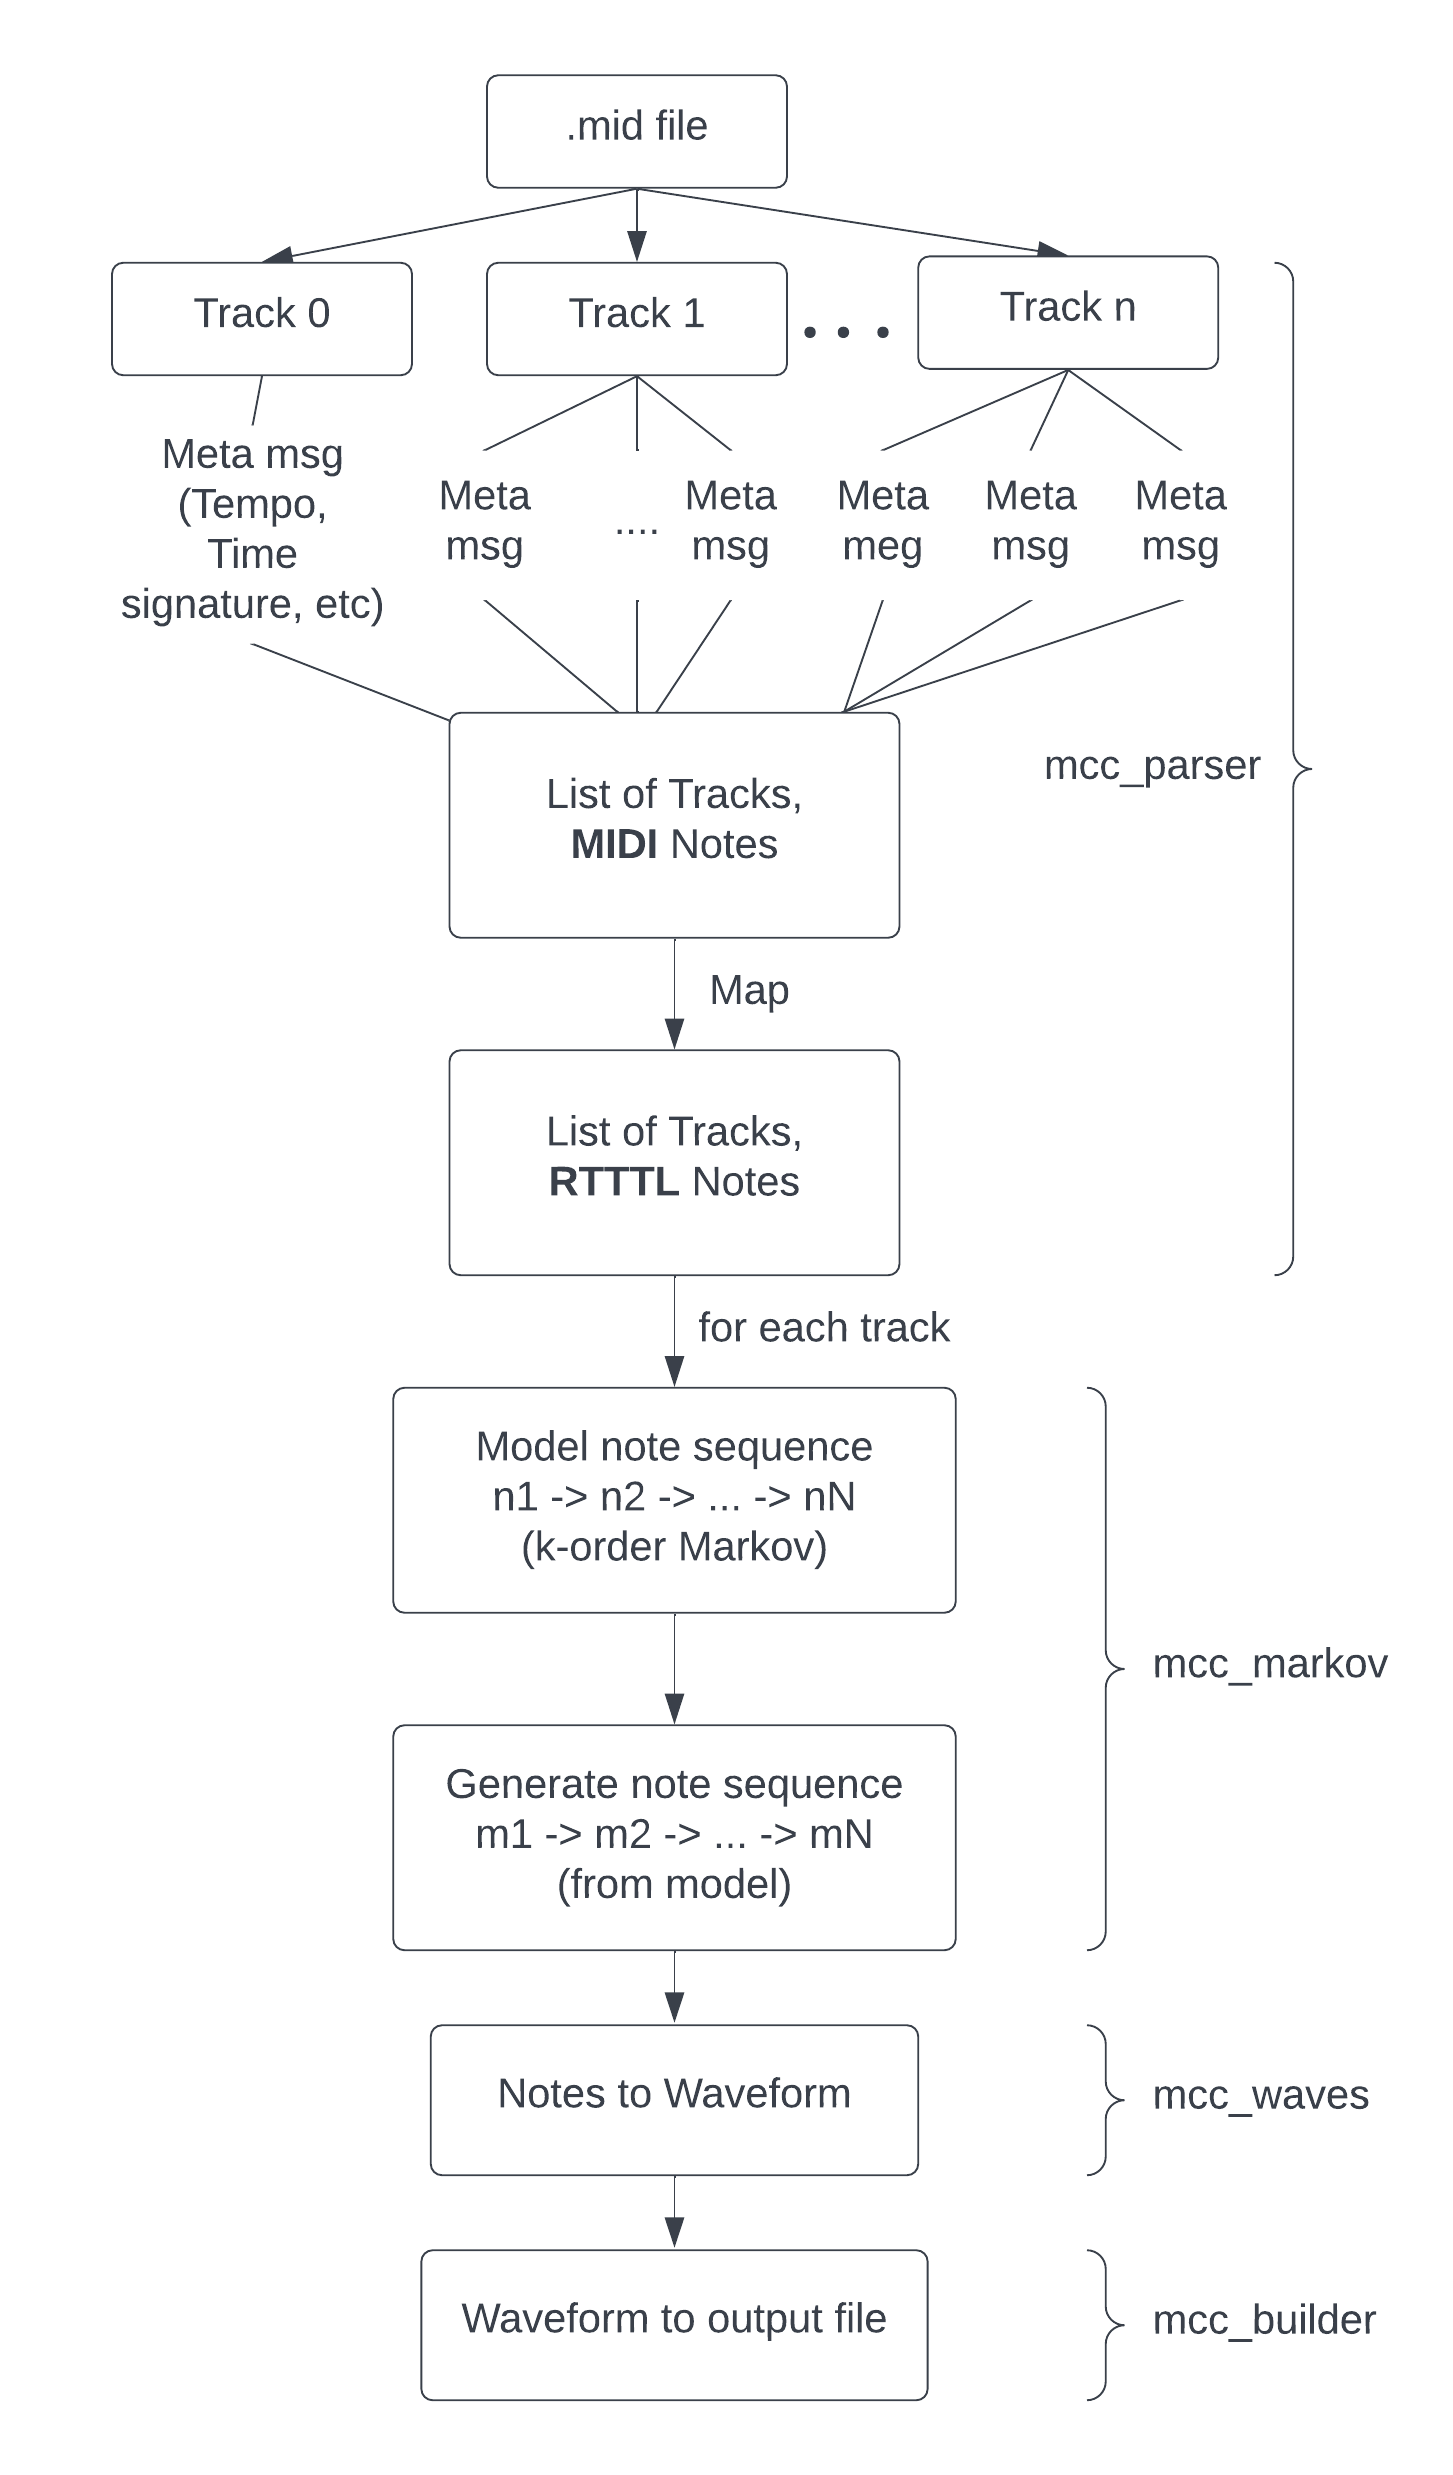
\includegraphics[width=230pt]{figs/roadmap.png}} \\

\subsection{Implementation}
So far, we have completed the mcc-parser module. It is the first module to convert our MIDI file to RTTTL string. Colson worked on the most of parser module functions, which 
takes MIDI file and tracks as inputs can converts them into RTTTL strings so that we can play them. Jae implemented the MIDI-to-RTTTL function, which converts each MIDI note 
into a corresponding RTTTL note, which reflects given beats and tempo of the song as well. Oscar wrote two classes for Markov models in the mcc-markov module. We also used a
Python file we found on Github by user devxpy \cite{Midi_instruments}, which converts MIDI note and instrument numbers to the appropriate instrument names. This function was used to attach the
instrument name to each note, so that in the future, we could attempt to apply that instrument type to each track when generating music.

The first class, $SimpleMarkov$ is a naive construct for modelling only first-order Markov processes, as well as biasing the probability of the most likely action with a 
greedification factor $\varepsilon$. $KMarkov$ is designed to model first- and higher-order Markov processes, and is far more configurable and accurate in its output than 
$SimpleMarkov$ models. Both classes have two methods: fit and predict, to tailor the model to a given episode, and sample a fitted model, respectively. While both classes are 
implementated generically, they are designed to model sequences of RTTTL notes as states. Each track of a MIDI file is modelled as a separate chain, and sampled independently. 
Higher-order Markov chains (i.e. $k>2$) generate reasonably good-quality music that, with a high enough $k$-value (e.g. $k>50$), come to resemble the original track. By itself, 
a single extended RTTTL track may not sound great, but we assume that once we gather all the MIDI tracks in a file and combine them all, the quality of the music will be much 
better. 

The next step would be to apply parser functions to a number of MIDI tracks simultaneously and combine them. The issue is with the starting times of each track. All 
of the MIDI tracks we have collected are type 1, which means they have multiple tracks with notes, but they all start simultaneously. The way the time attribute works in MIDI 
files is that it is a reference of time elapsed from the previous message, rather than a time of that message being played. In other words, A message with $time = 0$ starts 
immediately, and the following message that has $time = 100$ plays 100 ticks (MIDI units of time) after the previous message. Herein lies the issue with multiple tracks. 
Often the melody, harmony, bass, and so forth, don't play immediately (i.e. at $time = 0$) when the track starts. This causes an issue when combining the generated tracks 
back together, as the starting time is not saved anywhere. A solution we will explore is to look at the first message of each track and analyze the time value. This value 
can be converted to seconds, and saved as a value for each track. After generating the notes for each track, that value can be attached at the start, so that each track picks 
up at the same appropriate start time. 

We have completed export function as well, which converts the sound data into WAV file. After all those above tasks are over, If we have time, we would like to implement a 
GUI as well as it can makes the experience more intuitive. 

\subsection{Reflection}
Communication between the teammates was well done. After task delegation, each team member mostly worked on each of their task individually. Whenever someone was stuck or had 
a question, there was another person who could help out. We made steady progress as well, which is why we are keeping up with the deadlines that we set up initially. We expect 
to at least complete our project's "expected" goal by the end of the semester.

One challange that we faced was the format of MIDI file was not so intuitive. Especially, the time attribute is not the time for that given message, rather, it represent
time elapsed since the last note. We found some conflicting documentation on this matter, causing roadblocks of confusion. In order to achieve our goal, we had to make some 
compromise when parsing the MIDI notes, such as ignoring overlapping notes. Another challenge was we did not make a lot of pregress during the reading break, due to 
copious reading, as well as playing video games.

The followings are our scenarios for possible outcomes:
\begin{enumerate}
  \item \textbf{Basic/minimum}: single track RTTTL notes to chiptunes generator/extender. (Accomplished)
  \item \textbf{Expected}: MIDI file input of chiptune music with multiple tracks, generates and extends each track, outputs a WAV.
  \item \textbf{Stretch goal}: tunable model with GUI.
\end{enumerate}

% END

% Add bibtext citations to the file `refs.bib`.
\bibliography{refs}
\end{document}
